A Interface de Periféricos Serial, ou SPI (\emph{Serial Peripheral Interface}) nada mais é do que um dispositivo periférico usado na transmissão e recepção serial de dados. Porém a SPI é uma comunicação síncrona, ou seja necessita de uma fonte de clock de referência para se estabelecer além de um sinal de \emph{chip select}, ou \textbf{CS}, para ativar a recepção de dados no dispositivo receptor. Uma das principais características deste neta comunicação é o fato de que a comunicação em um dado barramento é unidirecional e de que se faz necessário no minimo três vias de comunicação.

\subsection{Padrão da Comunicação}

A comunicação SPI possui a maior taxa de transmissão, ou \emph{baud-rate}, dentre os demais protocolos de comunicação usados em microcontroladores, podendo chegar a até a 66Mpbs em periféricos com o AT45BD0100D da Adesto. O que possibilita um  \emph{baud-rate} tão elevado é o fato de que nesta comunicação a recepção e a transmissão de dados é feita separadamente e de forma direta, sem a necessidade de se transmitir bits de inicio ou termino de transmissão, e ainda de modo que o controle da transmissão é realizado pelo sinal CS (Chip Select) e pelo sinal  CLK (Clock).  A figura \ref{fig:SPI} apresenta o padrão de uma comunicação SPI.

\begin{figure}[H]
	\centering
	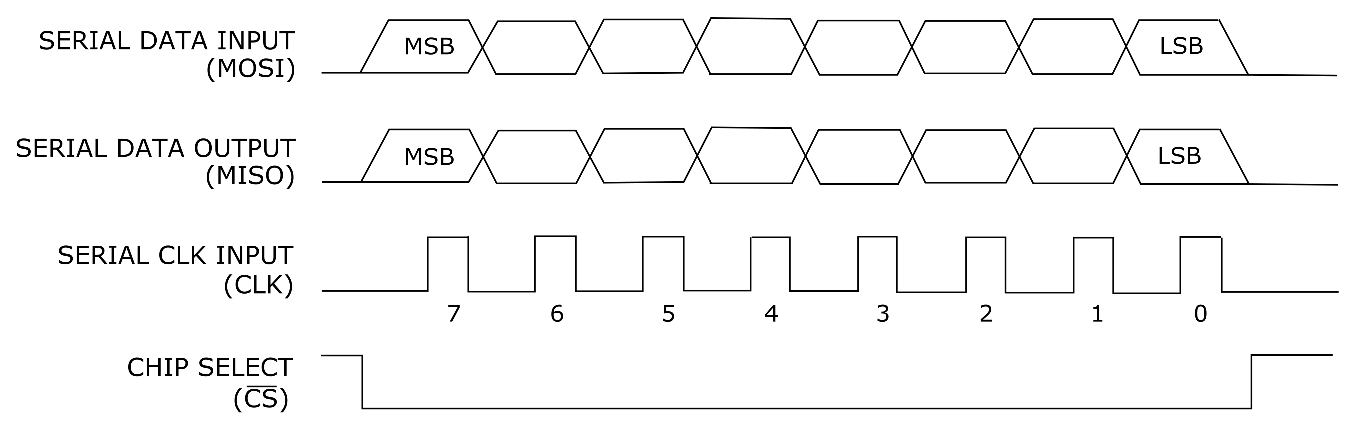
\includegraphics[width=1\textwidth] {figuras/PadraoSPI.eps}
	\caption{Padrão de Comunicação SPI}
	\label{fig:SPI}
\end{figure}

Para transmitir um dado de um dispositivo \textbf{Mestre} para um \textbf{Escravo} é necessário que o \textbf{Mestre} ative o sinal de CS do \textbf{Escravo} e fornecer a ele o sinal de clock de referência. Em seguida bit a bit deve ser transmitido pela porta MOSI \emph{Master Output - Slave Input} de ambos os dispositivos. 

Quando for necessário transmitir um dado de um  \textbf{Escravo} para um \textbf{Mestre}, novamente o \textbf{Mestre} deve ativar o sinal de CS do  \textbf{Escravo} e fornecer a ele o sinal de clock de referência, porém o dado será transmitido bit a bit pela porta MISO \emph{Master Input - Slave Output} de ambos dispositivos. 

\begin{figure}[H]
	\centering
	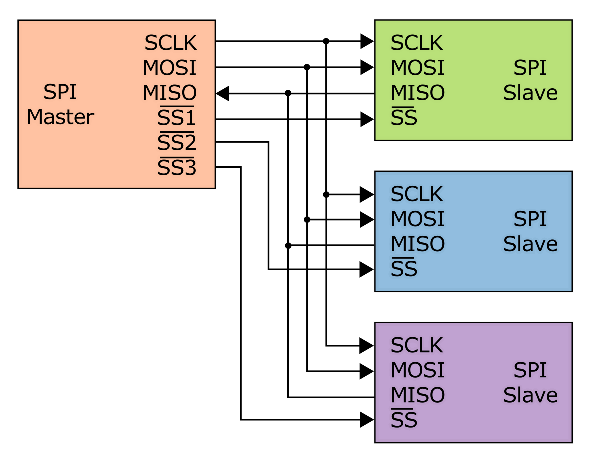
\includegraphics[width=0.6\textwidth] {figuras/BarramentoSPI.eps}
	\caption{Diagrama de Comunicação SPI - Vários Escravos}
	\label{fig:SPIDiagrama}
\end{figure}

A figura  \label{fig:SPIDiagrama} apresenta um diagrama básico de uma comunicação entre \textbf{Mestre} e vários \textbf{Escravos} através dos de barramentos de dados e de clock em comum.  

\subsection{SPI do TM4C1294NCPDT}


\subsection{Na TivaWare}